\documentclass{sig-alternate}

\usepackage{subfigure}
%\usepackage{multirow}
\usepackage[hyphens]{url}
\usepackage{graphicx}
%\usepackage[small,it]{caption}
\usepackage[noend]{algpseudocode}
\usepackage{algorithm}
%\usepackage{algorithmic}
\usepackage{amsmath}

%\usepackage{algorithm}
\DeclareMathOperator{\pContact}{p^\ast}
\DeclareMathOperator{\pTimeZone}{pTimeZone}
\DeclareMathOperator{\pStrangers}{pStgrs}
\DeclareMathOperator{\edges}{edges}
\DeclareMathOperator{\contactEdges}{contactEdges}
\DeclareMathOperator{\actEdges}{actEdges}
\DeclareMathOperator{\median}{median}
\DeclareMathOperator{\MLE}{MLE}
\DeclareMathOperator{\LCR}{LCR}
\DeclareMathOperator{\FriendLoc}{FriendLoc}
\DeclareMathOperator{\Backstrom}{Facebook}
\DeclareMathOperator{\p}{p}
\DeclareMathOperator{\haversin}{haversin}
\DeclareMathOperator{\Err}{Err}
\DeclareMathOperator{\AED}{AED}
\DeclareMathOperator{\ACC}{ACC}
\DeclareMathOperator{\quantile}{qntl}
\DeclareMathOperator*{\argmax}{arg\,max}
\renewcommand{\algorithmicthen}{}

\hyphenation{Four-square}
\hyphenation{Face-book}

\pdfpagewidth 8.5in \pdfpageheight 11in
\linespread{.97}

\newcommand{\jam}[1]{\emph{#1}}

\newcommand{\squishlist}{
\begin{list}
	{$\bullet$} { \setlength{
	\itemsep}{0pt} \setlength{\parsep}{3pt} \setlength{\topsep}{3pt} \setlength{
	\partopsep}{0pt} \setlength{\leftmargin}{1.5em} \setlength{\labelwidth}{1em} \setlength{\labelsep}{0.5em} } }
	
	\newcommand{\squishlisttwo}{
	\begin{list}
		{$\bullet$} { \setlength{
		\itemsep}{0pt} \setlength{\parsep}{0pt} \setlength{\topsep}{0pt} \setlength{
		\partopsep}{0pt} \setlength{\leftmargin}{2em} \setlength{\labelwidth}{1.5em} \setlength{\labelsep}{0.5em} } }
		
		\newcommand{\squishend}{
	\end{list}
	}


\frenchspacing

\begin{document}

\conferenceinfo{CIKM'13} {}
\CopyrightYear{2013}
\crdata{}
\clubpenalty=10000
\widowpenalty = 10000

\numberofauthors{1}
\author{
\alignauthor
For blind review
}

\title{FriendlyLocation: Using Tie Strength to Improve Location Estimation}

\maketitle
\begin{abstract}
We propose a novel network-based approach for location estimation in social
media that integrates evidence of the \textit{social tie strength} between
users for improved location estimation.
%
Concretely, we propose a location
estimator -- FriendlyLocation -- that leverages the relationship between the
strength of the tie between a pair of users, and the distance between the pair.
%
Based on an examination of over 100 million geo-encoded tweets and 73 million
Twitter user profiles, we identify several factors such as the
number of followers and how the users interact that can strongly reveal the
distance between a pair of users.
%
We use these factors to train a decision
tree to distinguish between pairs of users who are likely to live nearby and pairs of
users who are likely to live in different areas.
%
We use the results of this decision tree as the input to a maximum likelihood
estimator to predict a user's location.
We find that this proposed method significantly improves the results of
location estimation relative to a state-of-the-art technique.
Our system reduces the average error distance for 80\% of Twitter users from 40
miles to 21 miles using only information from the user's friends and
friends-of-friends,  which has great significance for augmenting traditional
social media and enriching location-based services with more refined and
accurate location estimates.
%
\end{abstract}

\jam{define contacts --- are defined to be the set of a user's friends, followers, and
people who a user mentioned in her tweets (i.e., people the user speaks to).}

\section{Introduction}
Location-based social media is widespread, with the adoption of voluntary
user-based location sharing via ``check-in'' services like Foursquare,
geo-tagged posts on Twitter, and photos shared on Flickr and Instagram.
%
These services allow users to annotate their activities with a location field,
ranging from a broad descriptor like ``New York'' or ``USA'' to an extremely
granular latitude/longitude pair  derived from the GPS capabilities of modern
smartphones.
%
Millions of users have already adopted these location sharing services,
providing an unprecedented \textit{geographical perspective} on the trails and
connections among millions of social media users.

By investigating the interplay between geography and social media, both
researchers and practitioners are enabling new applications that leverage
location.
%
Location information is increasingly incorporated into social media for
providing localized content, location-aware recommendations, and other
geo-spatial enabled services.
%
For example, researchers have begun investigating techniques to cluster users
based on their revealed geographic patterns \cite{scellato2010distance},
automatically deriving location-based social networks, and improving friend
suggestion based on geographic proximity \cite{cranshaw2010bridging},
\cite{wang2011human}, \cite{crandall2010inferring}.
%
Localized social media activity -- like Twitter discussions about a recent city
council vote -- can be automatically detected and directed to interested
parties.
%
Crowds of co-located people can be identified and related support services can
be directed toward them -- in the case of a fire or emergency, resources may be
more smartly targeted to the affected regions.

Tempering this excitement, however is a key challenge: how to derive
high-quality location estimates for users in social media.
%
Many users choose not to reveal their location, while others may reveal their
location only using noisy or overly general descriptors (e.g., `` New York'').
%
 To tackle this challenge, one of the most popular location estimation methods
 is \textit{network-based estimation}, in which a user's location is derived
 from the known location  properties of other users nearby in the social
 network (e.g,.
%
if most of my direct friends are in San Francisco, then perhaps I am as well)
\cite{davis2011infer}, \cite{li2012towards}.
%
One of the best known network-based approaches was introduced by Facebook
researchers Backstrom et al.
%
\cite{backstrom2010find} in a comprehensive study over 2.9 million Facebook
users.
%
This Facebook study analyzed users who had posted a home street address and
found that as distance increases, the probability of friendship decreases.
%
Building on this observational study of Facebook users, they showed how the
street addresses of a user's friends could be used to predict a user's location
within 25 miles 57\% of the time.

While an encouraging first step, this Facebook approach may encounter
difficulties in location estimation when applied more broadly to other social
media services:

\begin{itemize}
\item \textit{Multiple (often imprecise) location granularities.} First, many
    users in social media reveal broad, imprecise locations (e.g., at the city
    or state level), while others provide fine-grained latitude-longitude
    information.  In particular, users are less likely to post precise
    locations such as street addresses on public websites such as Twitter.  How
    can these multiple location granularities be integrated to account for
    uncertainty at different levels?
\item \textit{Varying social ties.} Second, not all relationships in social
    media are the same.  Some ties are stronger than others, and presumably
    some ties are more revealing of a user's location.  How does this variable
    tie strength nature impact location estimation?
\item \textit{Conflicting purposes.} Finally, many social systems serve
    different purposes.  Twitter, for example, is both a social network
    connecting friends (which may tend to be local) as well as a news media
    (supporting global dissemination)  \cite{kwak2010why}.  What is the
    appropriate balance between these conflicting purposes for location
    estimation?
\end{itemize}


To address these challenges, we propose a novel network-based approach for
location estimation that
  integrates evidence of the \textit{social tie strength} between users for improved location estimation,
  naturally incorporates uncertainty across multiple location granularities,
  and can distinguish between users of the system that operate at cross-purposes.
We investigate this approach through an examination of over 100 million
geo-encoded tweets and 73 million user profiles collected from Twitter.
%
Concretely, we propose a location estimator -- FriendlyLocation -- and
investigate the relationship between the strength of the tie between a pair of
users and the distance between the pair.
%
Based on this investigation, we identify several factors such as number of
followers and how the users interact that can strongly reveal the distance
between a pair of users, and use these factors to train a tree classifier to
predict the distance between a pair of connected users.
%
We use the results of this classifier as the input to a maximum likelihood
estimator to predict a user's location.
%
We find that this proposed method significantly improves the results of
location estimation relative to the Facebook technique.
%
FriendlyLocation improves the average error distance for 80\% of Twitter users
from 41 miles to 21 miles which has great significance for augmenting
traditional social media and enriching location-based services with more
refined and accurate location estimates.

\section{Related Work}
The study of geographical properties of online social media users has drawn
intensive attention in recent years.
%
Characterizing network properties in relation to local geography has been
studied in \cite{yardi2010tweeting}.
%
Lindqvist \cite{lindqvist2011mayor} analyzed how and why people use location
sharing services, and discussed the privacy issues related to location sharing
services.
%
User behavior with regard to the location field in Twitter user profiles has
been studied in \cite{hecht2011tweets}.

Scellato et al.  \cite{scellato2011socio} used data from three location based
social networks to investigate the relationship between distance and location,
and they showed that connections are not purely caused by geographical or
social factors.
%
They investigated two random models where they shuffle the user locations and
another where they shuffled the social connections and investigated what
happened to the user location.
%
They showed that if a user has more connections, then their friends tend to be
further away.
%
They also found that longer connections are equally likely to be part of a
social triangle as shorter connections.

Several researchers in recent years have looked into predicting user locations
in a social network based on the social graph.
%
In the largest-to-date study on this subject, Facebook researchers analyzed the
physical distance between Facebook users' social relations and utilized the
locations of a user's friends' to predict the user's geographical location
\cite{backstrom2010find}.
%
Davis et al. \cite{davis2011infer} investigated a system that predicted
location by taking a vote among the locations of the user's friends and picking
the most popular location.

An alternative to network-based approaches is \textit{content-based}, in which
a the content associated with a user either explicitly reveals location
information (e.g,. mentioning a local attraction like Disneyland) or implicitly
does so (e.g., by inferring subtle local linguistic cues to estimate a user's
location).
%
Cheng et al. \cite{cheng2010you} proposed a content-based system for locating
users on Twitter.
%
They found words that are highly concentrated in specific regions and built a
model to calculate the probability that a user lives at a location.
%
Eisenstein et al. \cite{eisenstein2010latent} proposed a functionally similar
system based on a latent variable model that predicted a user's location based
on the words in their tweets.
%
Recently, Li et al. \cite{li2012towards} proposed a system to integrate both
network and content-based estimation via a unified discriminative influence
model which combined locations that a Twitter user mentioned with the locations
of the user's followers.

In recent work \cite{sadilek2012finding}, the authors look at users who post at
least 100 geo-located tweets a month in NYC and LA.
%
They reconstruct the social graph from co-occurring geo-located tweets and used
dynamic Bayesian networks to predict where a user was at a particular moment in
time.

Finally, Cranshaw et al. \cite{cranshaw2010bridging} tackled the inverse of the
problem we are investigating: they predicted the existence of a social network
tie given precise location information from laptops and cell phones.
%
They used a collection of features of when users are co-located.
%
Together, these efforts have begun to lay a foundation for the study geo-social media.

\section{Location Estimation Incorporating Tie Strength}
In this section, we build a model for the probability that a user, who we refer
to as the target user, lives at a specific location given the approximate
location of his friends and followers.
%
Every user on Twitter has a set of people that they interact with, which we
refer to as their contacts.
%
This includes the user's friends, followers, and people they mention in tweets
(i.e., people the user speaks to).
%
Many of these contacts share their locations.
%
We define $L^c$ to be the set of known locations of the contacts of a user.
%
Given a target user, our goal is to estimate the location $l$ of the user
provided only with some imperfect information about the location of that user's
social network, $L^c$.
%
We first describe the baseline Facebook model for location estimation, identify
several limitations of applying it more widely, and then describe the proposed
FriendlyLocation approach that integrates tie strength for augmented location
estimation.

\subsection{Baseline: The Facebook Model}
The Facebook model developed by Backstrom et al. \cite{backstrom2010find}
begins with a striking observation: that the probability of friendship is
roughly inversely proportional to distance.
%
Specifically, by examining the ratio of actual edges at a particular distance
to the total number of possible edges at that distance (i.e., the probability
of friendship), they find a curve of the form $a(b+x)^{-c}$, with an exponent
close to $c=-1$.

With the empirically observed probability of friendship, they can estimate the
likelihood that a user lives at a location $l$ using both $L^c$, the set of
locations of the user's friends with known locations, and $L^s$, all 2.9
million known locations of Facebook users.
%
Then, the Facebook model estimates the likelihood of location $l$ as:
\[
    \Backstrom(l,L^c) =
        \prod_{l^c \in L^c} {\p(|l-l^c|) \over 1-\p(|l-l^c|) }
        \prod_{l^s \in L^s} 1-\p(|l-l^s|)
\]

\noindent where $\p$ is the probability of friendship given an input distance
(which again, can be derived empirically).
%
The first product in the formula combines the probabilities from a user's friends.
%
Locations near a user's friends will have a higher probability because $\p$ is
roughly inversely proportional to distance.
%
The last product in the likelihood formula is only a function of the location
$l^c_i$ and the locations of the strangers; it does not depend on any other
information about the target user's contacts.
%
For convenience, we refer to this as $\pStrangers$:
\[
    \pStrangers(l) = \prod_{l^s \in L^s}1-p(|l-l^s|)
\]

\noindent As suggested in \cite{backstrom2010find}, this can be pre-computed
for every location.
Major cities have the lowest probability for
$\pStrangers$, and remote areas have the highest probability.  It may seem
counter-intuitive that areas with low population density have a higher
probability, but consider this example: if someone has ten friends in New York
City and ten friends in a small town in upstate New York, they are more likely
to live in the small town, and just happen to know people in the big city.


The Facebook model naturally aggregates the locations of a user's friends, and
gives the probability that a user lives at a given location.
%
They then calculate this probability at each of the locations of the user's friends.
%
The location with the highest probability is often the center of the cluster of
the user's friends.
%
However, directly applying this approach to other non-Facebook domains may
encounter difficulties.
%
First, the Facebook empirical study focused only on the continental US, meaning
that distances between contacts were naturally limited to around 1,000 miles.
%
When investigating global friendships (as on Twitter or on the rest of
Facebook), there is considerable noise introduced in the 1,000--10,000 mile
range due to the distribution of land and oceans on the surface of the earth.
%
Second, the Facebook dataset had street addresses for approximately 2.9 million
Americans, and they used the friendships between users with street addresses to
do the calculation.
%
Since information on Facebook is usually only shared with a user's friends,
people are more willing to divulge their home addresses.
%
On most other social media websites, the location is publicly shared.
%
In practice, many users in social media reveal broad, imprecise
locations (e.g., at the city or state level), while others provide fine-grained
latitude-longitude information.
%
Third, the strength of connection between users necessarily varies, so
capturing this variation is important.
%
Encouragingly, Gilbert \cite{gilbert2009predicting} have shown how the strength
of a tie can be predicted by interaction patterns.
%
Finally, many social systems serve different purposes.
%
Twitter, for example, is both a social network connecting friends (which may
tend to be local) as well as a news media (supporting global dissemination)
\cite{kwak2010why}.

\begin{figure}[tb]
\centering
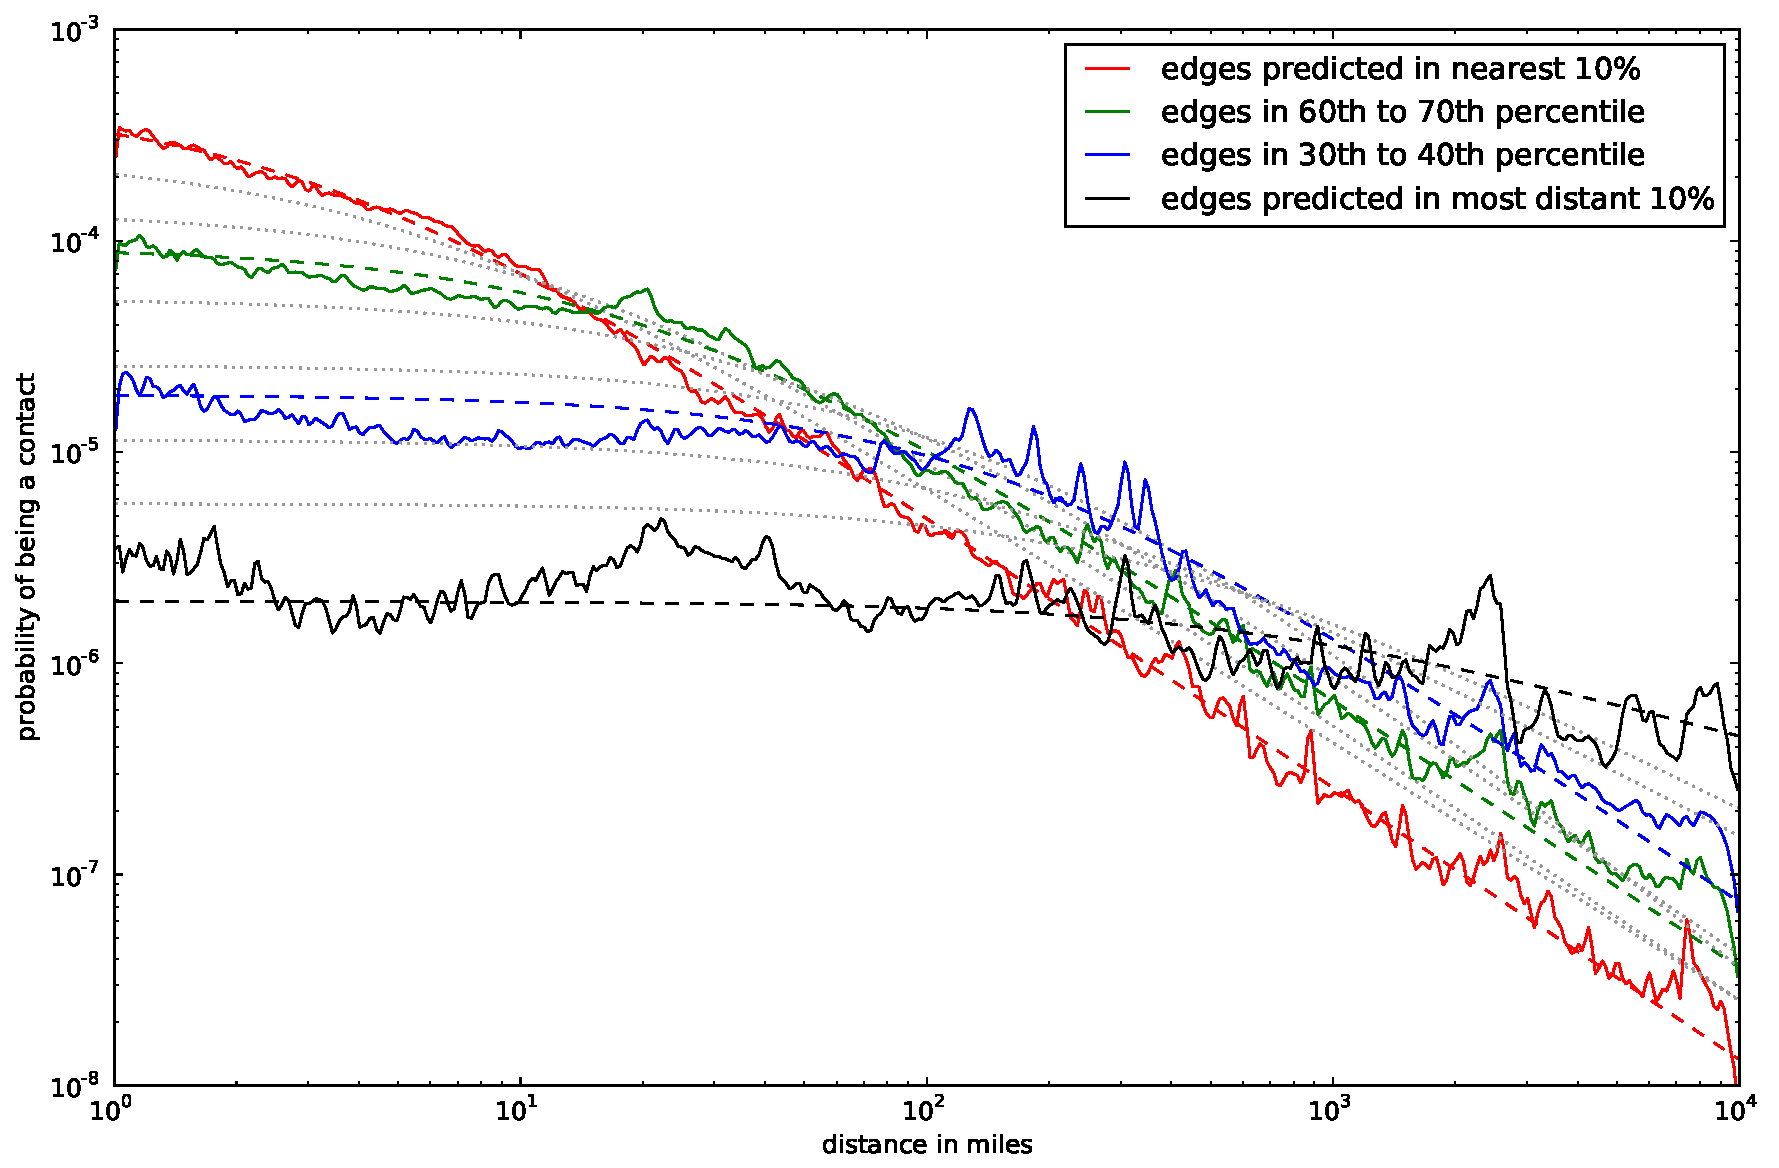
\includegraphics[width=.9\linewidth]{figures/vect_fit.pdf}
\caption{
After splitting edges into groups based on their predicted distance, each group
was fit to a curve.
%
Here are four of the ten curves and their curves of best
fit.
%
The other six curves of best fit are shown as faint dotted lines.}
\label{fig:NearProbFit}
\vspace{-2pt}
\end{figure}



\begin{table*}[tb]
\scriptsize
\centering
\begin{tabular}{l l p{4cm} p{6cm}}
    Label & Size & Description & Data obtained \\
    \hline
    Target Users & 249,584 & Users who posted at least 3 geo-located tweets &
    Location from GPS coordinates, user ids of friends and followers,
    and text of tweets. \\
    Geocoded Users & 894,617 & Users who posted at least 3 geo-located tweets
    and had a location the geocoder could parse, but not selected as target users &
    Location from GPS coordinates and geocoded location from user profile \\
    % 10,081,957 located contacts
    Located Contacts & 10 million & 25 contacts of target users with locations, randomly selected &
    Geocoded location from profile, user ids of friends and followers, and text of tweets \\
    % 71,596,805 leafs minus some of 250k contacts
    Leafs & 71 million & 100 contacts of target users, randomly selected &
    user profile (some of these users have a geocoded profile)\\
\end{tabular}
\caption{Four different sets of users and the data we obtained about them}
\label{tab:datasets}
\end{table*}


\subsection{FriendlyLocation: Incorporating Tie Strength}
A common theme of these challenges is that the quality of the geographic
information conveyed by a relationship in social media varies.
%
Some edges may convey strong evidence of the location of a user.
%
For example, intuitively the many edges between a user with an unknown location
and his co-workers (for whom we know their location) should contribute strongly
to the likelihood that the user is nearby those co-workers.
%
In contrast, links between a user with an unknown location and with a news
service (e.g., CNN) should contribute little discriminating power to estimating
the location of the user.

The challenge here is to separate the best contacts, who are likely to be
nearby, from bad contacts who are likely to be far away.
%
Simply encoding our intuitions about who should make a good contact is a
starting point, but could miss many non-obvious relationships: for example,
there may exist a pair of users who are good friends, communicate with each
other, have many friends in common, and yet still live on opposite sides of the
globe.
%

\jam{define Dp, Da, and n}

Hence, we propose to assess the relative quality of each edge from a target
user to his contacts, so that edges conveying strong location information are
weighed more than others.
%
This could be looked at as a classification problem where we want to classify
edges as local or non-local, but the problem is there is a smooth continuum
from local to non-local, and semi-local friends can be useful for location
prediction.
%
As a result, we model this as a regression problem, and we propose improving
the Facebook system by adding in information from a decision tree.
%
Concretely, suppose we have a single edge from a user to one of his contacts.
We propose to assign this edge to a quantile based on its estimated
``goodness'' as determined by the decision tree.
%
This decision tree will give us a set of $n$ predicted lengths $d^p_i \in D^p$
that correspond to the $n$ actual lengths of the edges $d^a_i \in D^a$.
%
Suppose we construct a set of $m$ quantiles, representing edges at different
predicted distances.
%
Let the boundaries for these quantiles be $\{q_0,\dots,q_m\}$,
where:\footnote{The notation used for order statistic may need some
    explanation.  $X_{(n)}$ is the $n^{th}$ element in the set $X$ when sorted
    in increasing order, so $X_{(2)}$ means the second smallest element in
$X$.}
\[
    q_j =
    \begin{cases}
        D^p_{(1+\lfloor {jn\over m} \rfloor)}, & j<m \\
        \infty & j=m
    \end{cases}
\]
\noindent The quantile for a specific distance $d^p_i$ can be found by
comparing it to the boundaries:
\[
    \quantile(d^p_i) = \max_{j \in \{0,\dots,m\}} \{j: d^p_i<q_j\}
\]

Hence, we can identify the actual edges ($\actEdges$) that exist with a distance of $d$.
%
This lets us find $\actEdges$, which is the number of users who fit in a
quantile $j$ and had an actual distance of $d$
\[
    \actEdges(j,d) = |\{
            i \in \{1,\dots,n\} :
            d=d^a_i \wedge j=\quantile(d^p_i)
        \}|
\]

By comparing the number of edges that could have existed to the number of edges
that actually exist at a specific distance and in a specific quantile, we can
find the probability that a contact at a specific distance is in a quantile:

\jam{define edges}
\[
\pContact(j,d) = \frac{\actEdges(j,d)}{\edges(d)}
\]

We can combine this improved model into the existing estimator by
replacing the probability of being a contact based purely on distance ($p$) to
the probability based on the regression tree ($\pContact$).
%
We now have a formula for predicting the best location given $L$, the set of
locations of the contacts, and $P$, the set of predicted distances to the same
contacts:
\[
    FL(l,L,P) =
        \left(
            \prod_{l^c_k \in L,p_k \in P}
            {\pContact(\quantile(p_k),|l-l^c_k|) \over (1-p(|l-l^c_k|))}
        \right)
        \pStrangers(l)
\]

\jam{This was commented out, but it defines edges...
Location prediction with a maximum likelihood estimator requires an estimate of
the probability that a user lives at a specific location.
%
We can find that probability by comparing the distribution of Twitter users to
the distribution of the contacts.
%
First, we need a model for the density of Twitter users.
%
We calculate the distance between every target user and every contact (even for
contacts and users who had no relationship).
%
We call the number of target and contact pairs that are $d$ miles apart
$\edges(d)$.
}

% i index in R, decision tree tuples
% j index in Q, quantile boundaries

Next, we need to model the probability that two users are contacts.
%
We ran the decision tree regressor on millions of edges to create a set of
tuples $R = (d^a_i, d^p_i)$ for $d^a_i \in D^a$ and $d^p_i \in D^p$ where
$d^a_i$ is the actual length of the edge, and $d^p_i$ is the value predicted by
the decision tree.

\jam{confusion about curve-fitting}
For each of the quantiles, we can fit $\pContact$ to the curve from
\cite{backstrom2010find}:
\[
    \pContact(j,d) = a_{j} (b_{j}+d)^{-c_{j}}
\]

We choose to split into ten quantiles, which gave us ten different curves for
the probability that a certain type of contact exists between a pair of users.
%
Four of the ten curves from one of the folds from the five-fold evaluation and
their lines of best fit are shown in Figure~\ref{fig:NearProbFit}.
%
The best contacts are orders of magnitude more likely to live near a target
user than the worst contacts.
%
If the predictions from the tree regressor were ignored, and users were placed
into one group instead of ten equal groups, this would reduce to the model for
friendship and distance presented in \cite{backstrom2010find}.
%
We choose ten because it was large enough to distinguish between the curves.
%
Larger numbers of quantiles give no benefit since the curves we are fitting
are so noisy as can be seen in Figure~\ref{fig:NearProbFit}.


\section{Factors Impacting the Length of an Edge}
In the previous section, we formalized the location estimation problem
incorporating evidence of tie strength.
%
But what factors actually impact the length of an edge? In this section, we
empirically examine a large sample from Twitter, totaling 100 million
geo-encoded tweets and 73 million user profiles.
%
Based on this sample, we examine the following properties to study how various
types of edges correlated with proximity, including
    (i) friendship relationships,
    (ii) friend and follower counts,
    (iii) conversations between users,
    (iv) if the account is public or private,
    (v) edges in social triangles,
    (vi) distances from a contact to their contacts, and
    (vii) granularity of locations.

\subsection{Data Collection from Twitter}
To investigate how social relation and geographical distance between the
relations correlate, we sample a dataset from Twitter.
%
Our analysis and prediction is based on data collected from Twitter during
May, June, and July of 2012.

We built a crawler to find these contacts for users who used Twitter's Location
Feature to disclose their location.
%
The crawler sampled over one hundred million geo-coded tweets by monitoring
Twitter's public streaming API for all of May 2012.
% 118,464,320 lines including keepalive newlines and non-status messages.
We kept the tweets from the users who posted at least three tweets, which left
us with 1,758,101 Twitter users.
%
For each of these users with geo-coded tweets, we used the median latitude and
median longitude of the locations of the user's tweets as an approximation of
her home location.
%
Some Twitter accounts, such as accounts that posted jobs, would
move around faster than a human could possibly move.
%
To account for this, the crawler calculated the distance between each tweet and
the user's home location.
%
The crawler ignored users if the median distance from their tweets to their
home location was greater than 50 miles.
%
This only removed 3.4\% of the geo-located users.
%
We also removed an additional 2.9\% of the geo-located users who did not have
any contacts with locations we could decode, which left us with 1.6 million
Twitter users with a known location.
%
We randomly selected 249,584 of these users for analysis and experimentation.
\footnote{We originally selected 250,000 users, but had to remove 416 of them.
These users had contacts with locations, but none of their contacts had
meaningful locations.}
%
We refer to these users as the target users.
%
Almost all of the experiments in this paper are based on these target
users.

Users who post geo-located tweets are not entirely representative of the
average Twitter user.
%
In particular, they are less concerned about their privacy and have a precise
location.
%
We only use information obtained from the contacts, and not the geo-located
users themselves in our prediction.
%
There are some Twitter accounts, such as large organizations, who do not have a
single location.
%
In practice, a location prediction system would need to identify users who do
not have a location.



% distribution of the contacts
%     med  avg      std
%rfrd 62.0 132.7148 278.394
%jfol 35.0 143.4844 456.629
%jfrd 78.0 153.5700 241.222
%jats  5.0   7.0764   8.060

For all of the target users, our crawler used Twitter's API to download
the users' 100 most recent tweets, a list of friend ids, and a list of follower ids.
%
We also collected the user profiles for a sample of users who were two steps
away from the target users on Twitter's social graph.
%
In the end, we collected just over 73 million Twitter user profiles.
%
Table~\ref{tab:datasets} shows a summary of the data obtained from Twitter.
%
This data was used to do the analysis in the rest of this section.

\begin{figure}[tb]
\centering
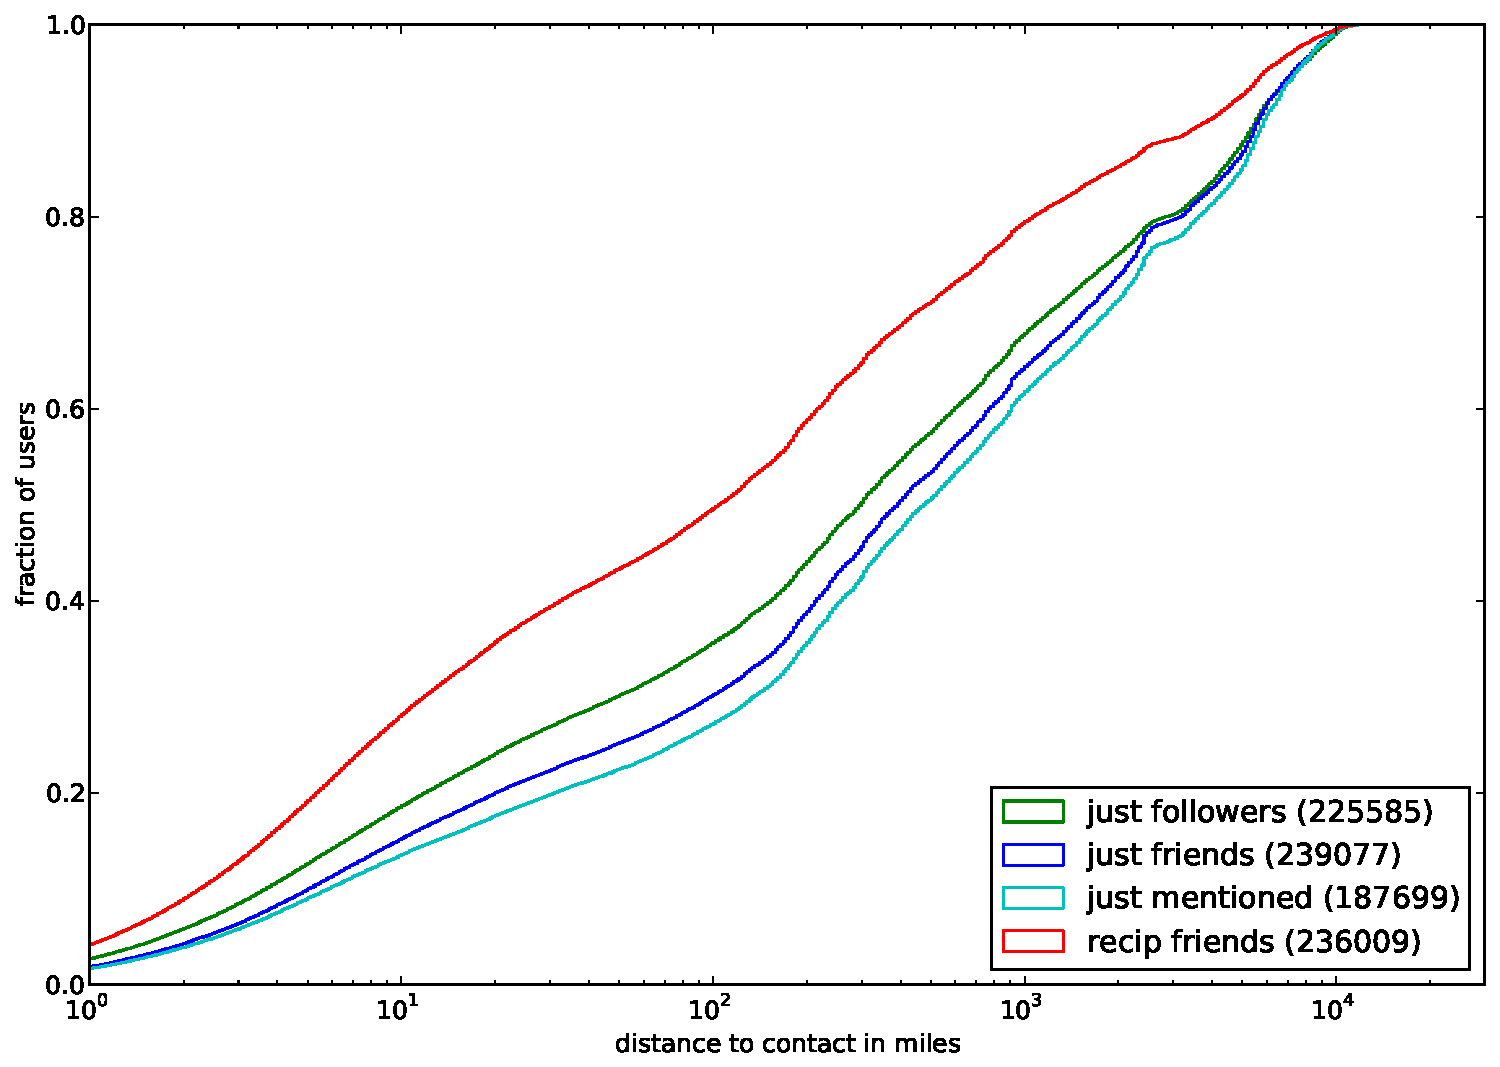
\includegraphics[width=.9\linewidth]{figures/edge_types_cuml.pdf}
\caption{
CDF of distance from target users to users they have some contact
with.
%
Reciprocal friends tend to be closer than other types of friendships.
}
\label{fig:EdgeTypesCuml}
\vspace{-2pt}
\end{figure}


\subsection{Factor 1: What type of contact is closest?}
\label{sec:EdgeTypes}
We first consider the type of contact and its impact on distance by dividing
all contacts into one of four disjoint sets:

\jam{check captialization of terms}
\begin{description}
\item[reciprocal friend:] The target user follows this user and is followed
    back.
\item[just friend:] The target user follows this user and is not followed
    back.
\item[just follower:] The target user is followed by this user, but does
    not follow them.
\item[just mentioned:] The users do not follow each other, but the target
    user mentioned the other user in a tweet.
\end{description}

Figure~\ref{fig:EdgeTypesCuml} shows the cumulative distribution
function(CDF) of the distance between a target user and several types of
contacts.
%
Distance is plotted on a logarithmic scale to show both local and
global effects.
%
On a logarithmic scale, the contacts are fairly evenly distributed from being
nearby to being on the opposite side of the world.
%
%For reciprocal friends, the 1\textsuperscript{st} quartile, median, and
%3\textsuperscript{rd} quartile of the distances are 7.9 miles, 106 miles, and 720 miles
%respectively.
%
%There is a relatively flat section in all the lines around 3,000 miles.
%
%3,000 miles is longer than the distance between the east coast of the U.S. and
%the west coast, but shorter than the distance from the east coast of the U.S.
%to Europe, so there are few population centers that are this distance apart.

In general, we observe that reciprocal friends are the closest, followed by followers, friends,
and finally users who are just mentioned.
%
38\% of reciprocal friends live within 25 miles while only 18\% of users
who are just mentioned live within that radius.
%
While it may seem that since being followed by someone and following someone
should be identical, they are not.
%
Celebrity and news accounts on Twitter often have large numbers of followers,
but they normally do not follow a large number of users.
%
Since the target user is selected randomly, they are usually an average
user and not a celebrity.
%
If they follow someone, it might be a celebrity; however, if someone follows
them, it is probably someone who knows them.

\begin{figure}[tb]
\centering
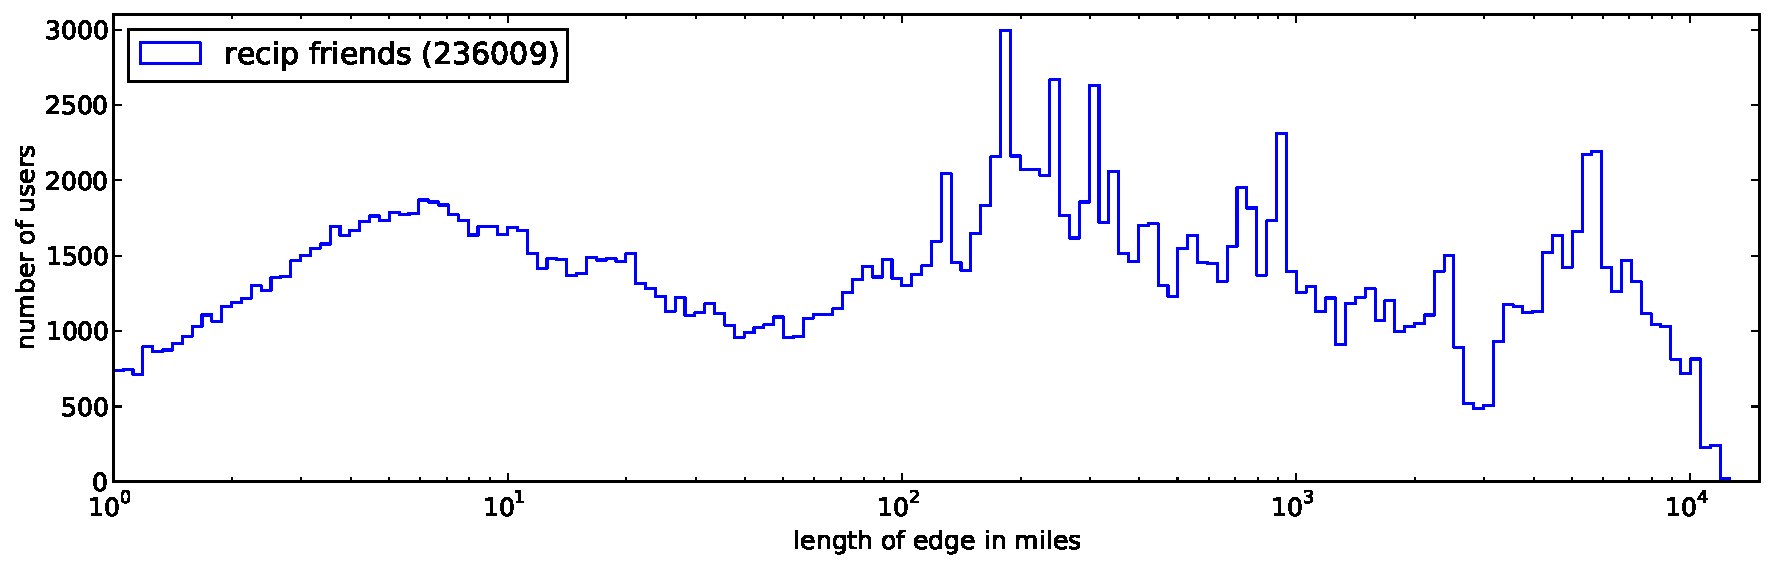
\includegraphics[width=.9\linewidth]{figures/rfrd_norm.pdf}
\caption{
Histogram of distance to reciprocal friends.
}
\label{fig:EdgeTypes}
\vspace{-2pt}
\end{figure}
\jam{is the EdgeTypes label right here?}


\noindent\textbf{What is the distribution of contacts?}
To further analyze the distribution of contacts, we show in
Figure~\ref{fig:EdgeTypes} a logarithmically-scaled
histogram of the distances between various types of contacts.
%
All four types of contacts follow roughly the same
distribution: one peak around 10 miles from people who live nearby, and several
other peaks between 100 and 10,000 miles.
%
Since the contacts often list the name of their town, there is a small distance
between the geocoded location of the town and the location of the target
user's tweets.
%
There aren't as many contacts in the 30 to 150 mile range, but then after 150
miles, peaks start appearing for major cities.
%
One reasonable explanation for this is that Twitter is not just a social
network; it is also a news distribution network as described in
\cite{kwak2010why}.
%
This distribution suggests that users have two types of contacts: people who
they met in real life, and people who they met online or know about via
mainstream media.

Most previous location prediction work has focused on doing predicting
locations in the continental U.S.
%
In the first figure from \cite{mcgee2011geographic}, McGee et al. observe a
bimodal distribution in distances between American Twitter users with strong
peaks at 10 miles and 2500 miles.
%
When looking at this similar set of data on a global scale, we find more chaos
in the distribution of contacts at distances greater than 200 miles.

\begin{figure*}[tb]
\centering
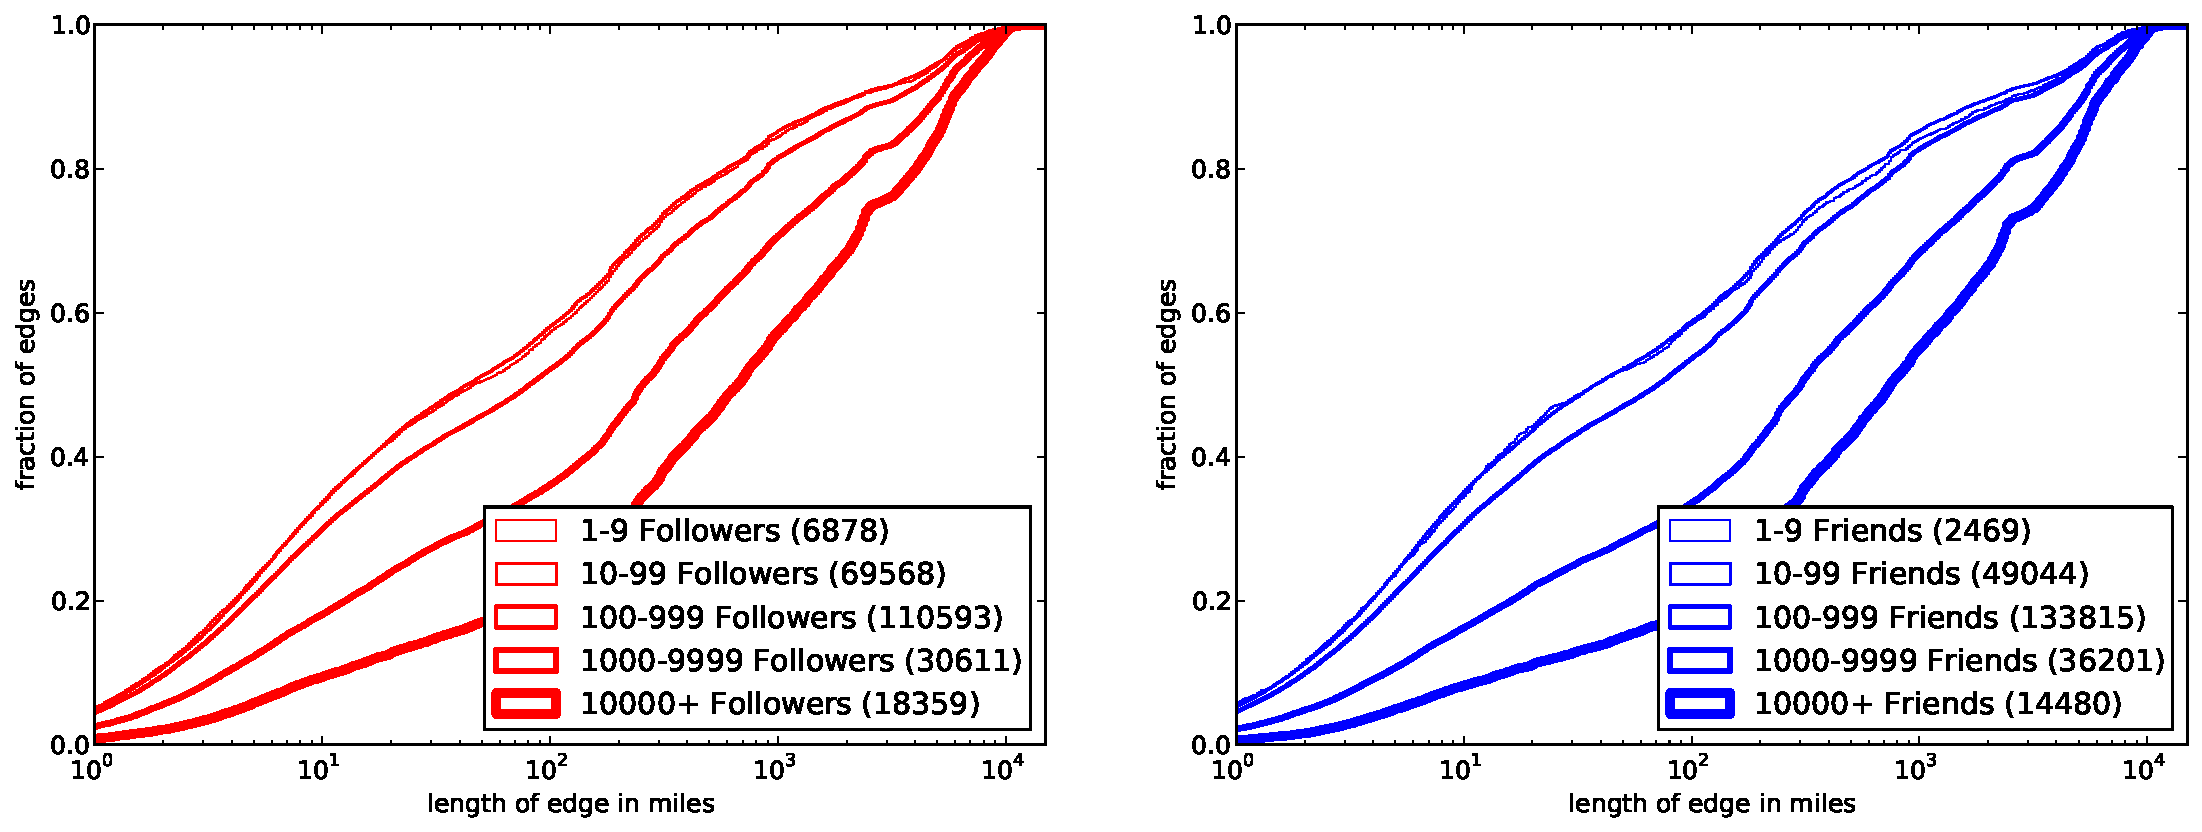
\includegraphics[width=\linewidth]{figures/edge_counts.pdf}
\caption{
A comparison between number of followers and proximity---people who have more
friends or followers tend to be further away.
}
\label{fig:EdgeCounts}
\vspace{-2pt}
\end{figure*}

\subsection{Factor 2: Does the number of friends and followers a person have affect how
close they are?}

The second factor we consider is the number of friends and followers of a contact.
%
%Since the primary goal of this research is to predict the location of users, we
%want to be able to discern the differences between contacts.
%
%When looking at number of friends and followers, we focus our attention on the
%number of friends and followers a contact has rather than the numbers for the
%target user.
%
We took each of the reciprocal friendships that we looked at in
Section~\ref{sec:EdgeTypes} and put them into five log-scaled bins based on
the number of friends or followers that the contact had.
%
Figure~\ref{fig:EdgeCounts} shows the result of this procedure.

In general, people who are more promiscuous followers and friends are less
likely to live nearby.
%
This makes sense because it is easy to meet 15 Twitter users in real life, but
very few people know 1000 Twitter users who live in the same town.
%
Contacts with 10--99 followers were within 25 miles of their geo-located friend
45\% of the time while contacts with 1000--9999 followers were nearby only 26\%
of the time.
%
There was a similar result in the number of friends: the proportion of local
contacts went from 46\% down to 23\%.

Mainstream media and celebrity accounts such as the New York Times and Lady
Gaga have millions of followers while normal users rarely have more than a few
hundred.
%
Follower count and friend count are good ways to distinguish celebrity and news
accounts which are useless for location prediction.


\begin{table*}[tb]
\scriptsize
\centering
\begin{tabular}{l | r r | r r | r r | r r | r r}
    & \multicolumn{2}{c}{both mention}
    & \multicolumn{2}{|c}{target mentions}
    & \multicolumn{2}{|c}{contact mentions}
    & \multicolumn{2}{|c}{both ignore}
    & \multicolumn{2}{|c}{overall} \\
    \cline{2-11}
    &local&count&local&count&local&count&local&count&local&count \\
    \hline
    recip friend & 42\%&28067 & 50\%&17903 & 45\%&21066 & 35\%&168973 & 38\%&236009 \\
    just follower & 40\%&2001 & 47\%&792 & 40\%&5958 & 25\%&216834 & 25\%&225585 \\
    just friend & 21\%&23314 & 40\%&910 & 42\%&1884 & 21\%&212969 & 21\%&239007 \\
    just mentioned & 18\%&182978 & 36\%&4721 & & 0 & & 0 & 18\%&187699 \\
\end{tabular}
\caption{
If target users interact with their contacts, then they are more likely to
live nearby.
}
\label{tab:ComTypes}
\end{table*}

\subsection{Factor 3: Are users closer to people they communicate with?}

We look at the 100 most recent tweets for the targets and one of their
contacts for each type of their contacts.
%
The edges are divided into groups based on whether the target user
mentioned the contact and whether the contact mentioned the target user.
%
For each of the groups, we calculate the percentage of contacts who
live within 25 miles of the targets and the number of edges in that group.
%
This is shown in Table~\ref{tab:ComTypes}.
%
Since contacts who were just mentioned were mentioned by the target
user by definition, the contact mentions and both ignore table cells are
empty.

In almost every case, increased communication increases the probability that
two users live near each other.
%
There is one exception: when an average user mentions someone they follow who
does not follow them back, it has no effect---in both cases the contact is
local 25\% of the time.
%
In other words, if a random user mentions a celebrity who does not bother to
reply, they probably do not live in the same area.
%
On the other hand, in the rare event that someone who is just a friend replies
to their follower, then the probability that they live near each other is much
higher---it goes from 21\% to 42\%.

The weakest type of contact is users who were just mentioned, but never
replied to.
%
If the person is mentioned, then 36\% of users with no
friend/follow relationship who have a conversation live within 25 miles.
%
This is approximately equal to the 35\% of reciprocal friends who ignore each
other and live within 25 miles.
%
Unsurprisingly, the strongest type of connection is reciprocal friends who
communicate.
%
One challenge to using communication patterns as a source of information for
location prediction is that the communication patterns that are correlated
with proximity are rare.

\begin{table}[tb]
\centering
\begin{tabular}{l | r r | r r}
    & \multicolumn{2}{c}{Public}
    & \multicolumn{2}{|c}{Private} \\
    \cline{2-5}
    &local&count&local&count \\
    \hline
    Recip Friend & 37\%&211136 & 41\%&24873 \\
    Just Follower & 25\%&204417 & 31\%&21168 \\
    Just Friend & 21\%&233849 & 39\%&5228 \\
    Just Mentioned & 18\%&183368 & 35\%&4331 \\
\end{tabular}
\caption{
    Comparison between public accounts and private accounts on Twitter.
    Private accounts tend to be closer.
}
\label{tab:EdgeTypesProt}
\vspace{-4pt}
\end{table}

\subsection{Factor 4: Are users closer to private accounts?}

Like many social networks, Twitter allows users to control the privacy settings
on their account.
%
The specifics differ from network to network, but in Twitter's case
a user can make their account private which means followers have to get
permission to follow the account.
%
There are demographic differences between public and protected accounts.
%
For example, Gilbert \cite{gilbert2008network} demonstrates that rural users
are more likely to make their accounts private than public accounts.
%
In the case of protected accounts on Twitter, basic information
about their profile such as their location and the number of friends and
followers is public, but their friends list, followers list, and the text of
their tweets is private, and not available for analysis.

As seen in Table~\ref{tab:EdgeTypesProt}, the most dramatic difference between
private and public occurs if a user follows a protected account.
%
Since users generally only allow people they know to follow a protected
account, this brings the users almost as close together as if they were
reciprocal friends.
%
On the other hand, if a protected account follows the target user, they
are only slightly more likely to be nearby.

\begin{figure}[tb]
\centering
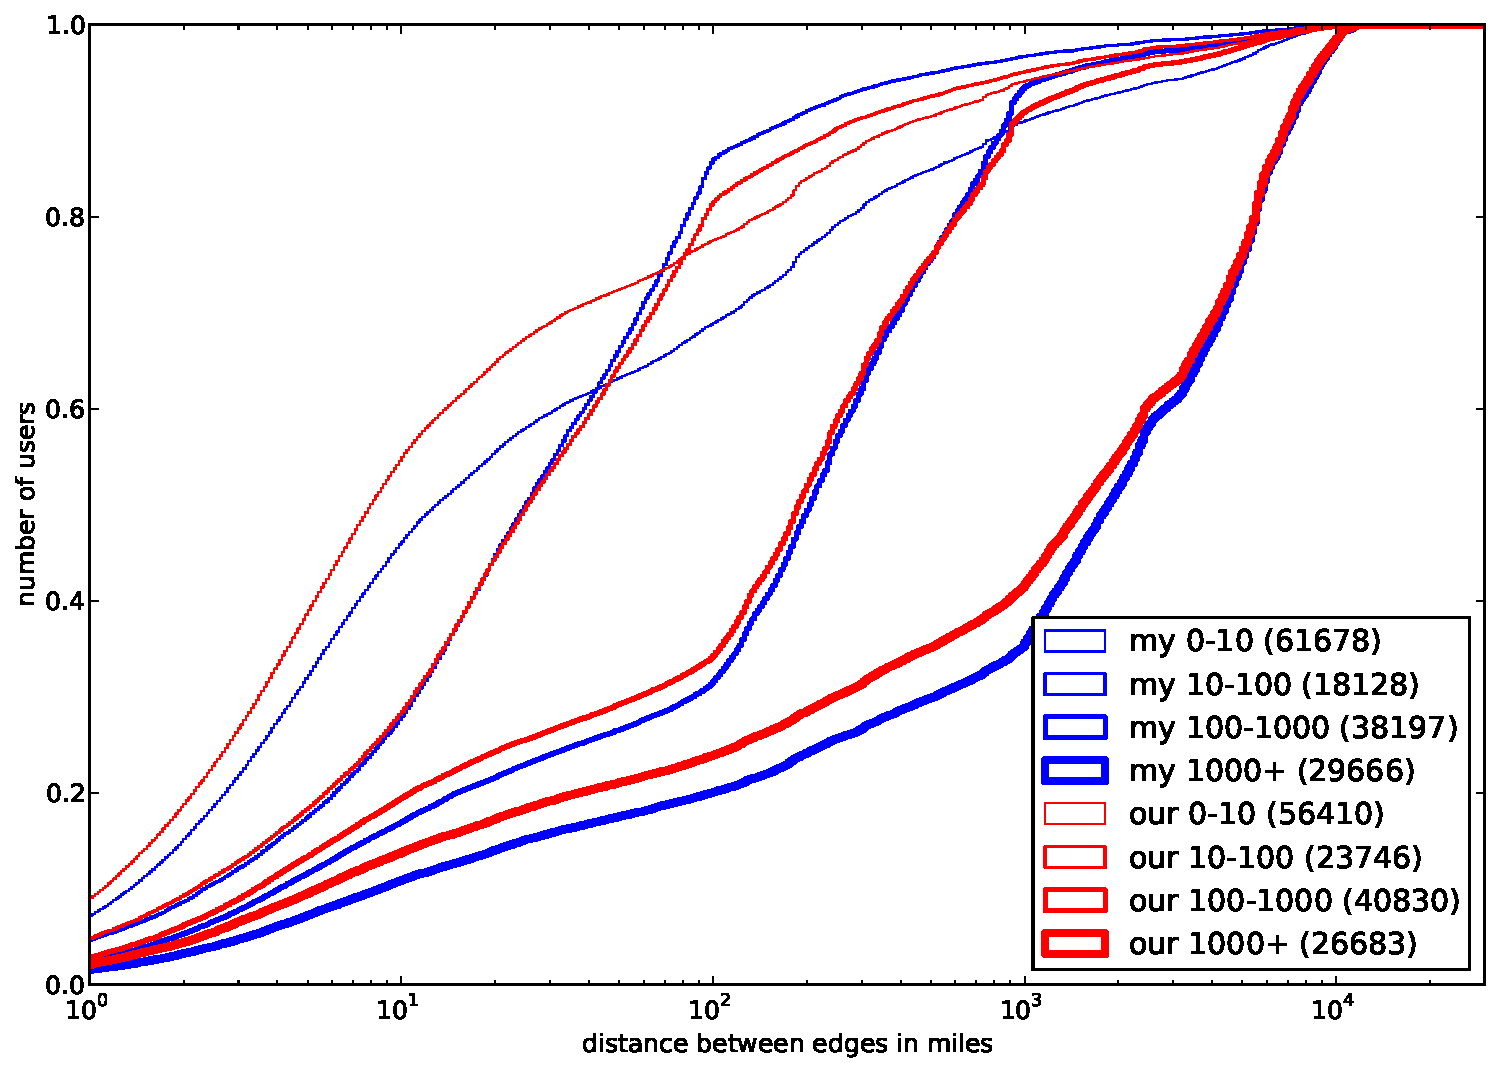
\includegraphics[width=.9\linewidth]{figures/near_triads.pdf}
\caption{
Comparison between distance to a mutual friend, labeled ``our'', and someone
who is not a mutual friend, labeled ``my''.
If two contacts are mutual friends and live near each other, a target user is
more likely to live near them than two contacts who live nearby but are not
mutual friends.
}
\label{fig:NearTriads}
\vspace{-2pt}
\end{figure}

\subsection{Factor 5: If two of your friends live near each other, does that increase the
chance they live near you?}

We now turn our attention to triangles of users.
%
Finding useful relationships between the edges of a social triangle is tricky
because the three distances depend on each other.
%
Unfortunately, it is fairly simple to show using the triangle inequality theorem
that if two users are 1000 miles apart, then the third member of the triangle
has to be at least 500 miles from one of the other two.
Since this isn't a useful result, we designed a more complex experiment to
analyze the relationship between the sides of the triangle.
A script searched for a specific pattern in the social network of
the target user's reciprocal friends: two people who were friends with each
other and a third person who had no connection with the other two:

\begin{center}
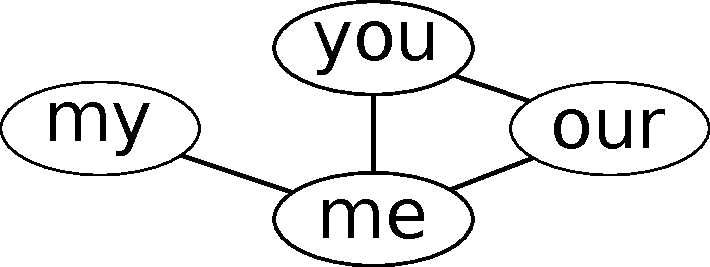
\includegraphics[width=0.3\linewidth]{figures/near_triads_dia.pdf}
\end{center}

To help label the four users, we describe this social graph from the
perspective of the target user:

\begin{itemize}
\item ``me'' is the target user
\item ``you'' is the contact who is reciprocal friends with ``me''
\item ``my'' has no relationship with ``you'' and is reciprocal friends with ``me''
\item ``our'' is reciprocal friends with both ``me'' and ``you''
\end{itemize}

We found this pattern for 147,669 of the target users.
%
If a user had multiple instances of this pattern, it picked one of them
randomly so that particular users would not bias the results.
%
%Since our crawler only retrieved friend and follower information for a few
%reciprocal friends per user, it is reasonable to assume that this pattern
%is more common, but the sample is more than enough data to draw some
%conclusions.
%
Figure~\ref{fig:NearTriads} shows a comparison between distances to the ``my''
users and the ``our'' users.
%
For each of the ``my'' users and the ``our'' users, we put them into one of
four logarithmically scaled bins based on their distance from the ``you'' user.
%
Then we plot the CDF for the distance from the target to the ``my'' and ``our'' users.
%
This allows us to investigate the effect of mutual friendship on distance.
We report one very simple result: if two of your friends are close (within 10
miles), then whether they know each other or not strongly affects how close
you are to them.
%
If they are farther apart, it doesn't matter.

\begin{figure}[tb]
\centering
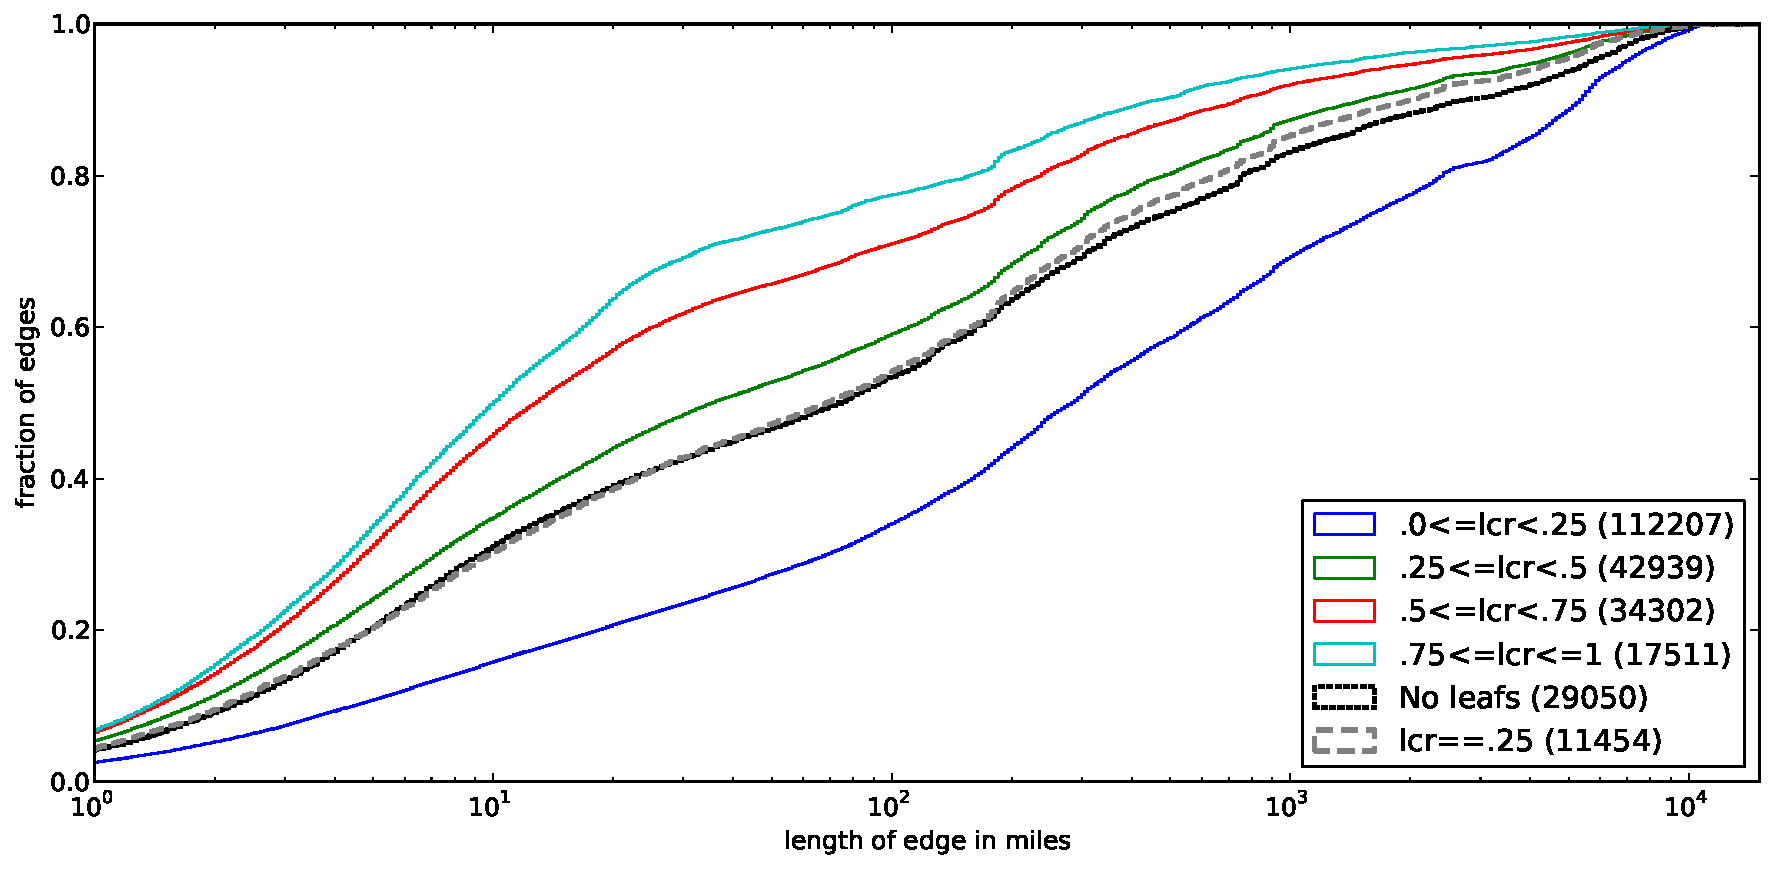
\includegraphics[width=.9\linewidth]{figures/locals_10.pdf}
\caption{
The colored lines show the distance to contacts split into groups based on the
proportion of the contact's friends and followers who live near the contact.
The dotted line shows the distance to contacts who have no locatable contacts.
%This graph is based on at most 10 leafs per contact.
Contacts who have a high proportion of nearby leafs are much more likely to
live near the target user.
}
\label{fig:Local10}
\vspace{-2pt}
\end{figure}

\begin{figure}[tb]
\centering
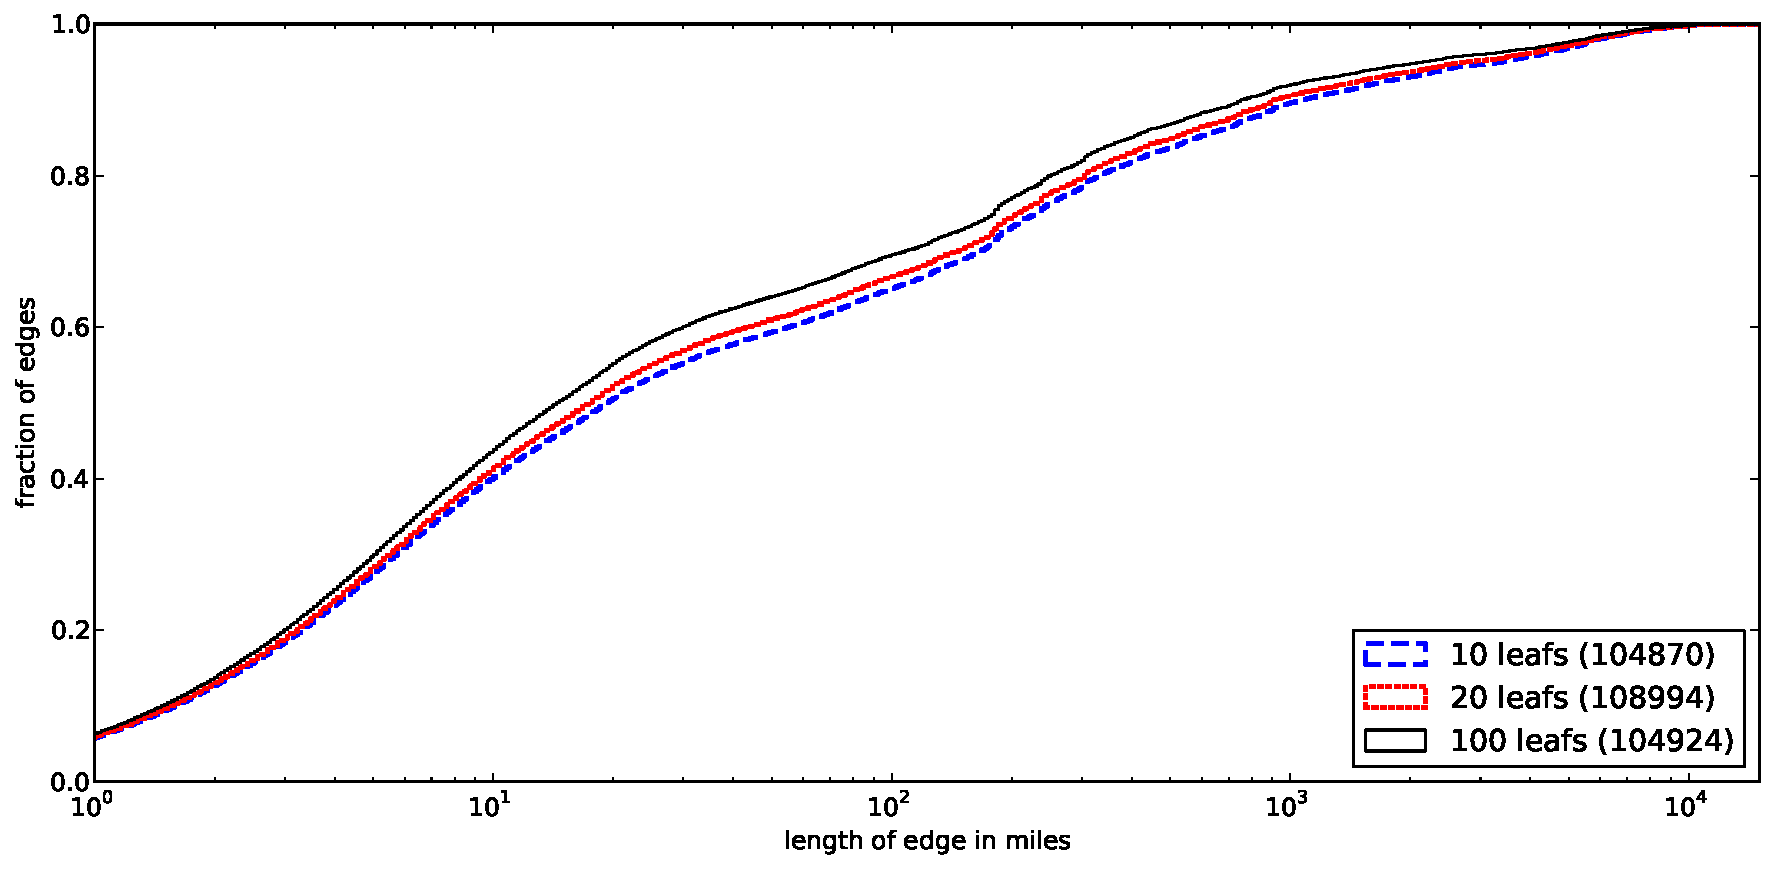
\includegraphics[width=.9\linewidth]{figures/locals_cmp.pdf}
\caption{
    Distances to contacts with a local contact ratio better than the median LCR
    for several numbers of leafs.
    Although looking at more leafs makes users with a high LCR more likely to
    be nearby, it probably doesn't justify how long it takes to compute.
}
\label{fig:LocalCmp}
\vspace{-2pt}
\end{figure}

\subsection{Factor 6: Are some users closer to all of their friends and followers?}
\label{sec:closer}

In the previous sections we only looked at the contacts of the target
users.
%
In this section we will go two steps out on the social graph and
investigate the friends-of-friends.
%
We want to know if some users are more localized than others, so we compare
contacts with lots of local contacts to contacts with mostly distant contacts.
%
\textbf{Local Contact Ratio}(LCR) is the fraction of a user's contacts
who live near the user.
%
For a contact at location $l^c$ and a set of their contacts' locations L, we
formally define LCR as follows:
\[
    LCR(l^c,L) = { |\{ l_i \in L : |l_i-l^c|<25 \}|
                    \over |L| }
\]
%
We picked a cutoff distance of 25 miles to distinguish between local and non-local
contacts.
25 miles is about the distance where the bulk of local users ends as seen in
Figure~\ref{fig:EdgeCounts}.
%
The distance cutoff is somewhat arbitrary, but it doesn't seem to matter much
in practice since we are really trying to distinguish between contacts who are
hundreds of miles away and contacts who live in the same town.
%
Around one in ten contacts did not have any contacts with a location from the
contacts we looked at---they were treated as a separate group.

In \cite{li2012towards}, the authors model the probability distribution of
user's followers using a Gaussian distribution, and use this to build a
location prediction system.
%
There are many other ways to analyze the leafs: average distance to the leafs,
median distance to the leafs, fitting the distances to a curve such as a
Gaussian.
%
We are looking at location prediction anywhere in the world, which means
contacts may be 10,000 miles away, and a location 10,000 miles away is nearly
as bad as a location 1000 miles away, so average is obviously not useful.
%
The disadvantage to using the median is more subtle.
%
As seen in Figure~\ref{fig:EdgeTypesCuml}, the median distance to a contact is
often in the 100--1000 mile range, and only about a third of contacts are
actually local.
%
This means that median distance to leafs does a reasonable job of separating the
worst contacts from the average contacts, but local contact ratio does a better
job of identifying the very best contacts.

\jam{check figure citation}
%Figure~\ref{fig:Local10} is a graph of the distance to reciprocal friends split
%into bins based on the local contact ratio of the contact.
%This shows that some users are much more local than other users.
%
The figure shows that some users are much more local than other users.
For example, a local newspaper may have thousands of followers and few friends,
but the people who follow a newspaper are generally local.
According to the other factors we looked at, the newspaper is a bad predictor
of location, but in reality it is a great predictor.

Of the factors we have investigated, this is the one that is most strongly
correlated with distance---in the next section we will see that local contact
ratio ends up at the top of a decision tree to separate local contacts from
non-local contacts.
%
One problem with this technique is that it is somewhat expensive to deal with
the large number of profiles two steps out on the social graph.
%
Our crawler originally looked at 100 leafs per contact because Twitter's API
will return up to 100 profiles at a time, but fetching and saving all those
profiles is slow.
%
In Figure~\ref{fig:LocalCmp}, we compare contacts with a high LCR calculated
using at most 100 leafs per contact to at most 10 leafs per contact.
%
The percentage of contacts within 25 miles with a good LCR based on 10 leafs,
20 leafs, and 100 leafs was 53\%, 55\%, and 58\%, respectively.
%
All of these are noticeably closer than reciprocal friends who are within 25
miles 38\% of the time.


\subsection{Factor 7: Are some locations better than others?}
The location field on a user's profile is just a text field that asks the user
to respond to ``Where in the world are you?''.
%
Responses include neighborhood names, state names, country names, and even
jokes and nonsense.
%
We use Gisgraphy
%\footnote{\url{http://www.gisgraphy.com/}}
to geocode this free-form text to a location using the GeoNames database.
%\footnote{\url{http://www.geonames.org/}}

Since some locations are significantly more useful than others, we needed a way
to evaluate the quality of a location.
%
The geocoding users are the 894,617 users who posted geo-located tweets, were not
selected as target users, and also filled in the the free-response location
field with something that the geocoder is able to decode.
%
We can compare the results of the geocoder to the location of the geo-located
tweets for these users to quantify how accurate the geocoder is for certain
types of locations.
%
We define the \textbf{location error} to be the great circle distance between a
user's home location (from their tweets) and the location returned from the geocoder.
The location error for a user can vary from less than a mile to over ten
thousand miles.
%
We calculated the location error for each of geocoding users, and grouped the
users by their location.
%
For the 17,370 locations that had at least three geocoding users, we calculated
the median location error (MLE) for that location.
%
All the users who were at locations with only one or two users were grouped
according to the type of location returned by the geocoder.
%
We calculated the median error for each location type.
%
The median is more appropriate than the average or standard deviation because
those metrics are strongly affected by large outliers.
%
%We choose to make the cutoff three because that is the smallest value where the
%median is not just an average.
%
This gives us a method to estimate the quality of a coordinate returned by
Gisgraphy.

\begin{figure}[tb]
\centering
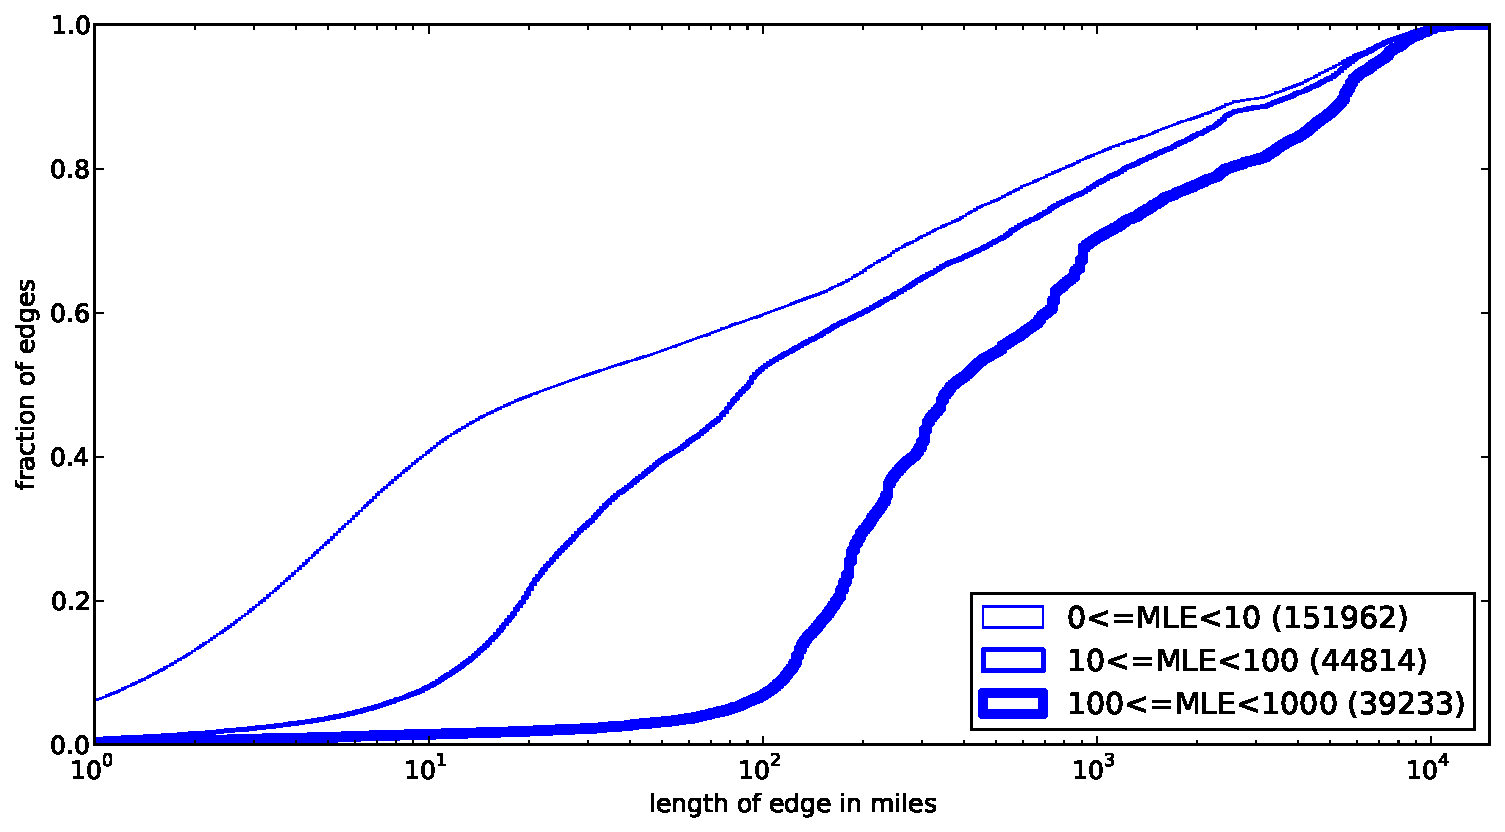
\includegraphics[width=.9\linewidth]{figures/rfrd_mdist.pdf}
\caption{
Reciprocal friends divided into groups based on the median location error(MLE)
of their location.
Contacts who report a location with a low MLE usually live near their contact,
while contacts with a high MLE generally live in the same region.
}
\label{fig:RfrdMdist}
\vspace{-2pt}
\end{figure}

Figure~\ref{fig:RfrdMdist} shows the length of edges to reciprocal friends
divided into three groups based on MLE.
%
Contacts with a low MLE provide relatively high-quality location
information---50\% of reciprocal friends with a MLE less than 10 live within 25
miles of the target user.
%
Contacts with locations with a MLE greater than 1000 were ignored for all of
the experiments in this paper, since these locations were almost always
nonsense values that happen to decode to an actual location.

\subsection{Summary}
Based on this large-scale analysis of Twitter, we conclude the following:

\begin{itemize}
\item Reciprocal friendships tend to be physically closer than contacts with
    less strong relationships such as someone who is just a follower.
\item Contacts who mention or are mentioned by the target user on Twitter tend
    to be located nearby.
\item Protected accounts tend to be closer, but we provide less additional
    information for assessing their relative quality.
\item Contacts with lots of friends and followers tend to be further away
    (since, in many cases these contacts correspond to celebrities or news
    organizations).
\item Some accounts, such as a local newspaper, may have lots of users from the same area.
    These accounts can be identified by looking at a small number of their contacts.
\item Contacts with more precise locations are more useful for location prediction.
\end{itemize}



\section{Building and Evaluating FriendlyLocation}

In this section, we integrate the observations from our study of the factors
that impact distance into the FriendlyLocation location estimator.
%
While there are many options for mapping from input factors to tie strength, we
adopt a decision tree regressor based on the CART algorithm (classification and
regression trees) to distinguish the best edges from the worst.\footnote{Since
    most of the input features are correlated and either binary or non-linear,
    linear regression is unlikely to work well.
    In addition, the data is dense and low-dimensional, so support vector machines
    do not work well.}
%
A decision tree regressor works similar to the well-known decision tree
classifier, except that it produces real numbers as output instead of discrete
classes.
%
During training, the training data is recursively split based on the input
variable with the most predictive power to build a binary tree.
%
Each of the internal nodes of this tree have a cutoff for one of the input
variables, and the leaves of the tree have a predicted value.


\begin{figure}[tb]
\centering
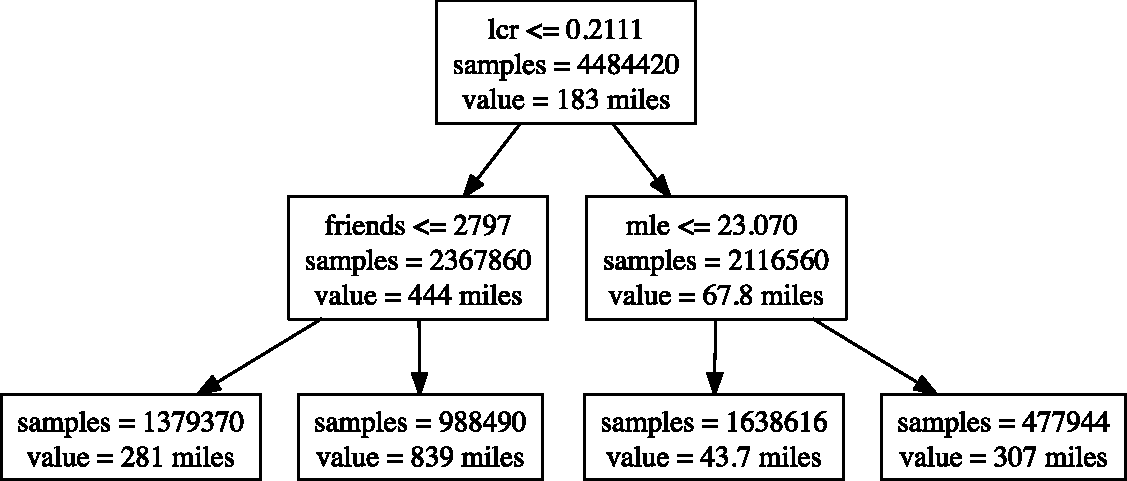
\includegraphics[width=.8\linewidth]{figures/tree_top.pdf}
\caption{
    \jam{What do samples and value mean in this chart?}
    The top three levels of the decision tree. This tree will predict a
    distance of 839 miles for a contact with a local contact ratio of .2 and
    2800 friends. It will predict a much-closer distance of 43.7 miles for a
    user with a local contact ratio of .5 and a median location error of 10
    miles.
}
\label{fig:TreeTop}
\vspace{-2pt}
\end{figure}

\noindent\textbf{Setup.} Since the distances between users varied by several
orders of magnitude, we trained the regressor to predict the log of the
distance.
%
The tree regressor was configured to not split leafs with fewer than 1000 data
points to prevent over-fitting.
%
The top three levels of a decision tree are shown in Figure~\ref{fig:TreeTop}.
%
The predictor does not do a great job of predicting the actual distance to a
contact; there's simply too much noise.
%
However, it does do an excellent job of separating the closest pairs of users
from the most distant pairs as we will show in the next section.



We evaluate the system against a baseline implementation, and we investigate
several modifications to the system.
%
We use five-fold cross validation on the target users to evaluate the system.
We evaluated the FriendlyLocation system against the 249,584 target users.

For each of the folds, we ran the tree classifier and generated a new set of
curves for $\pContact$ from the training data.
%
We did not recalculate $\pStrangers$ or the probability as a function of distance
used for the baseline, since these are fairly independent of the selected set
of users.

\noindent\textbf{Metrics.} We evaluate the system against the metrics used in
previous works: accuracy at 25 miles (ACC) which was used in
\cite{backstrom2010find} and average error distance (AED) proposed in
\cite{cheng2010you} and extended in \cite{li2012towards}.
%
Following the notational conventions from \cite{li2012towards}, we define ACC
and AED for a set of users $u \in U$ with $\Err(u)$ as the distance between a
target user's home location and the predicted location.

Accuracy is the fraction of users who live within 25 miles of their predicted
location:
\[
    \ACC(U) = { |\{ u \in U : \Err(u)\le25 \}| \over |U| }
\]

Average error distance (reported as AED@100\%) is as follows:
\[
    \AED(U) = { \sum_{u \in U} \Err(u) \over |U| }
\]

Since AED may be affected by outliers, we also report the AED at other
percentiles, following \cite{li2012towards}.
%
%The effect of outliers that they mention is even larger in our work than theirs
%because we are using locations from around the world instead of focusing on
%just the U.S.

\subsection{Evaluating FriendlyLocation}
We investigate several implementations of the FriendlyLocation system along
with two baseline systems, which we will discuss in upcoming sections:
\begin{description}
\item[Baseline] This is based on the maximum likelihood estimator presented in
    \cite{backstrom2010find}. Some changes to the system had to be made to make it
    work on Twitter's directed graph. (Facebook friendships are always
    reciprocal.)
\item[Nearest Contact] This predictor chooses the location of the contact that
    the tree regressor picks as the closest contact.
\item[FriendlyLocation Basic] This is the system described in the previous
    section with only information from the locations of contacts.
\item[FriendlyLocation - Strangers] This is the system described in the previous
    section without $\pStrangers$.
\item[FriendlyLocation - Leafs] This is the system described in the previous
    section without the locations of the leafs and tweets from the contacts.
\ifdefined\THESIS
\item[FriendlyLocation + Time Zone] This is the system described in the previous
    section plus the target user's time zone information.
\item[FriendlyLocation + Location] This is the system described in the previous
    section plus the target user's reported location is included in the
    estimation.
\fi
\end{description}

\begin{figure}[tb]
\centering
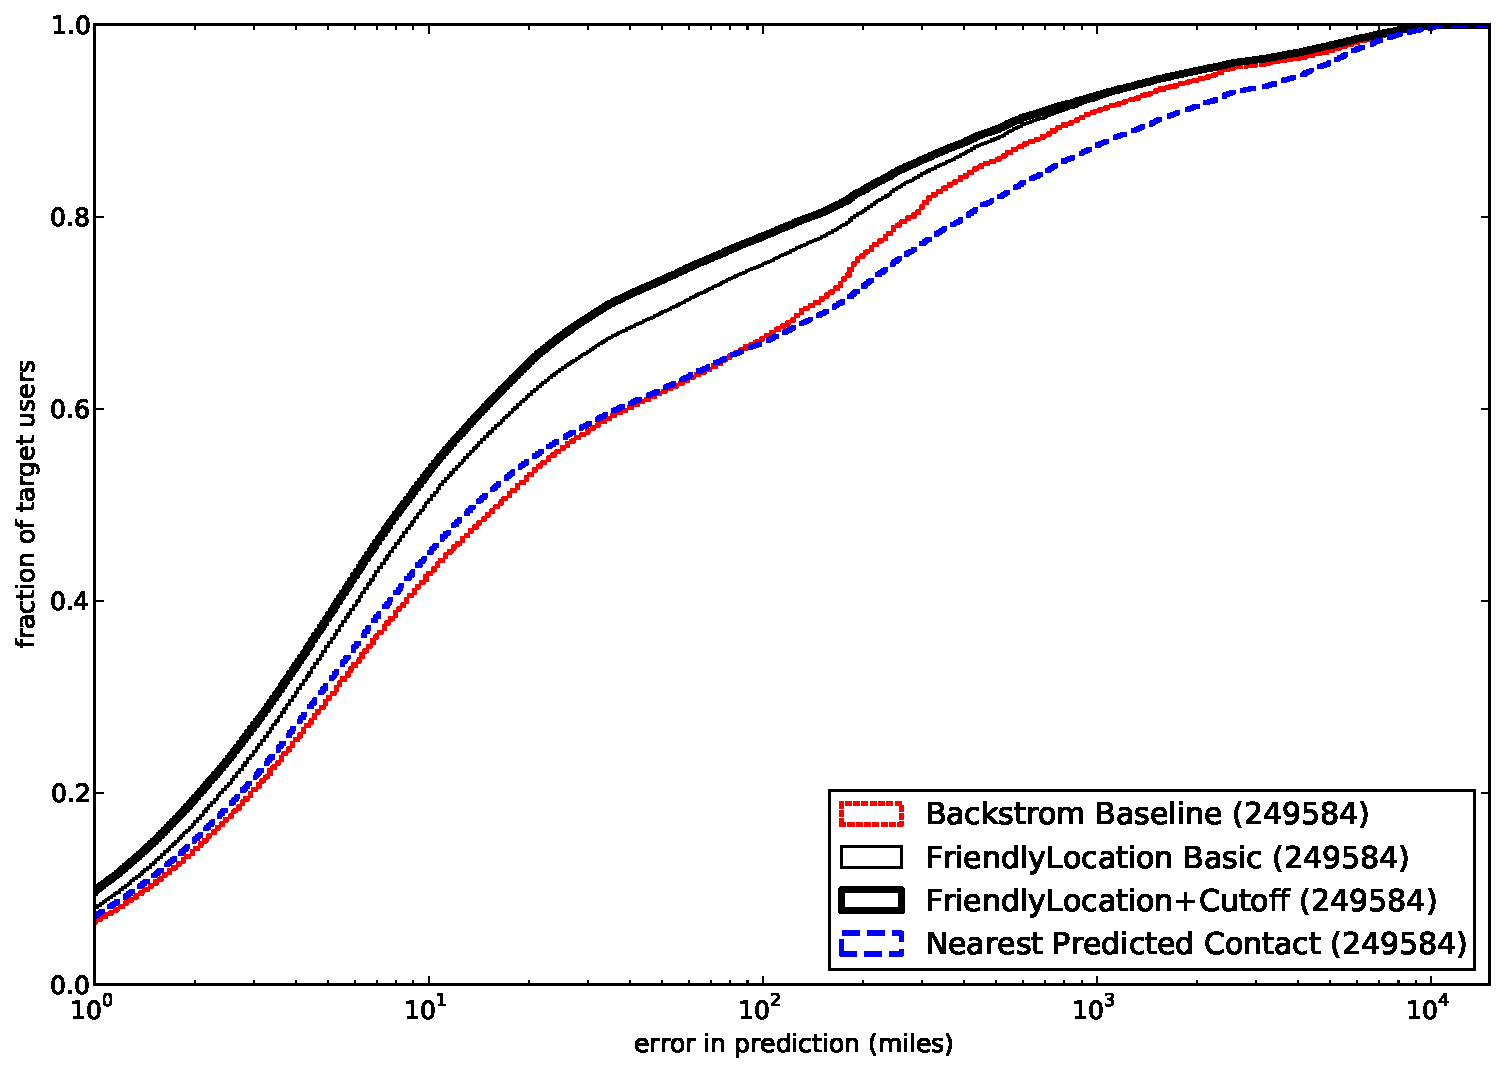
\includegraphics[width=.9\linewidth]{figures/fl_basic.pdf}
\caption{
    FriendlyLocation against several baseline systems.
}
\label{fig:results}
\vspace{-2pt}
\end{figure}

\begin{table}[tb]
\scriptsize
\centering
\begin{tabular}{l  r r r r}
    Model & aed@60 & aed@80 & aed@100 & acc@25 \\
    \hline
    Baseline & 8.41$\pm$.038 & 40.8$\pm$.20 & 426$\pm$3.9 & 55.7\%$\pm$.09\% \\
    Nearest & 7.73$\pm$.117 & 50.3$\pm$.39 & 594$\pm$9.3 & 56.5\%$\pm$.22\% \\
    FriendLoc$-$Strangers & 5.79$\pm$.028 & 25.2$\pm$.18 & 377$\pm$4.3 & 62.4\%$\pm$.09\% \\
    FriendLoc$-$Leafs & 5.36$\pm$.011 & 22.1$\pm$.12 & 367$\pm$4.0 & 63.6\%$\pm$.12\% \\
    FriendLoc Basic & 5.35$\pm$.008 & 21.4$\pm$.12 & 364$\pm$3.2 & 63.9\%$\pm$.05\% \\
\end{tabular}
\caption{
    Results of our location prediction system when compared to a baseline.
    The value after the $\pm$ is the standard deviation from the five-fold
    cross-validation.
}
\label{tab:results}
\end{table}



Table~\ref{tab:results} shows our system compared to a baseline implementation.
%
As seen in the table our basic FriendlyLocation system predicts the location
within 25 miles 63.9\% of the time.
%
Our basic system preforms significantly better than the baseline implementations.
%
The results are more impressive when you look at it in terms of average error
distance.
%
The baseline system has an average error distance of 40.8 for the best 80\% of
predictions, and our basic system has an average error distance of 21.4.
%
This means that our system is better at making good estimates better than it is
at making bad estimates good.
%
Unfortunately, when the predictor is wrong, it can be very wrong.
%
As seen in Figure~\ref{fig:results}, around a tenth of the predictions are worse
than 1000 miles for all of the predictors.
%
Some of this inaccuracy may be caused by inaccurate training data, but there is
no real way to know.





\subsection{Ignoring Strangers}
Calculating $\pStrangers$ is very expensive.
%
It only has to be computed once, but if you wanted to do location prediction on
a different social network, it would need to be recomputed.
%
We investigate the FriendlyLocation system without this information, by running
prediction without multiplying by $\pStrangers$ when calculating the overall
probability for each location:
\[
    \prod_{l^c_k \in L,p_k \in P} \pContact(\quantile(p_k),|l-l^c_k|)
\]
As seen in Table~\ref{tab:results}, removing this information results in a
slightly worse prediction.
%
There is a trade-off to be made here, and it may not be worth the time it takes
to calculate $\pStrangers$.

\subsection{Prediction Using Only Contacts}
Local Contact Ratio was the top node in the tree classifier for all 5 decision
trees, which means it was the most important feature for classification.
%
However, getting information about the leafs is by far the most expensive part
of the crawling and predicting process.
%
If we don't crawl the leafs, we also do not need to download the friends and
followers of the contacts to find the leafs, which makes the process well over
an order of magnitude faster.
%
We re-ran the tree regressor, curve fitting, and prediction using only
information from the target users friends, followers, and tweets and the
profiles of the contacts.
%
The accuracy for FriendLoc$-$Leafs at 25 miles was 63.6\% which is not quite as
good as the basic version of FriendLoc at 63.9\% accuracy, but they are still
very close.
%
Prediction using only contacts takes only four calls to Twitter's API instead
of the approximately 80 API calls it takes to do the basic version of
FriendlyLocation.

\section{Conclusion}

In this paper, we have demonstrated that some features of relationships are
correlated with physical proximity.
%
For example, users with lots of followers tend to be distant, while users who
mention each other tend to be closer.
%
In general, users with stronger ties tend to be local.
%
We used this to accurately predict the locations of users on a social media
website.

There are two general directions that the future work on this research could
go: improving the results of the prediction and using the predicted locations
to build systems.
%
One way to improve this predictor is to combine tie strength and the social
graph with other factors such as the words users choose to use as described by
Cheng et al.\cite{cheng2010you}.
%
It could be useful for the predictor to return not just a location, but an
estimate of the quality of the prediction.
%
The system described in this thesis only considered users who have a
well-defined location.
%
FriendlyLocation could be modified to identify users who do not have meaningful
locations such as people who constantly travel and accounts that represent
large organizations.

Finally, high-quality geographic information opens up new avenues for research
and software engineering.
%
Location prediction will allow websites to provide hyper-local content and
services.
%
For example, the distance between a pair of users could be considered when
suggesting new friends on a social network and websites will be able to give
users more accurate, localized search results.

The idea that started our research into location prediction was community crowd
detection.
%
With geographic location of users, we can cluster users and find local
conversations.
%
These conversations can be analyzed to understand local political and social
events.
%
Location prediction will allow us to create a more clear picture of the
conversations in a community.


%\fontsize{9pt}{10pt}

%
% The following two commands are all you need in the
% initial runs of your .tex file to
% produce the bibliography for the citations in your paper.
\bibliographystyle{abbrv}
\bibliography{fl}
% You must have a proper ".bib" file
%  and remember to run:
% latex bibtex latex latex
% to resolve all references
\end{document}
